\section{Prova da NP-Completude}

Para realizar a prova da NP-Completude de Zelda, vamos primeiro demonstrar que tal problema é
NP-Hard, reduzindo-o para o problema 3SAT. Depois, mostraremos que é NP. Como por definição o conjunto
de problemas NP-Completo é a intersecção dos conjuntos de problemas NP com o conjunto de problemas NP-Hard,
teremos provado que Zelda é NP-Completo.

\subsection{NP-Hard}

\newtheorem*{theorem}{Teorema 1}

\begin{theorem}
    É NP-Hard decidir quando uma posição final é alcançável a partir de uma dada posição
    inicial em uma versão generalizada de The Legend Of Zelda: A Link to the Past.
\end{theorem}


\begin{proof}
    Existem várias maneiras de demonstrar esse teorema, uma vez que se uma parte do jogo
    for NP-Completa, todo o jogo também será. Para isso, utilizaremos apenas baús de tesouro
    e blocos, que servirão como alvo do gancho (vamos assumir que Link começa com esse item).
    Para realizar a prova, basta descrevermos o ambiente do jogo de acordo com os dispositivos
    do framework apresentado. Como esse não é um jogo de plataforma, não precisamos de um dispositivo
    específico de começo e fim, podendo o começo ser uma posição arbitrária dentro de uma caverna
    (onde normalmente ficam os puzzles que precisam do gancho) e uma posição arbitrária do mapa aberto,
    respectivamente.
    
    O dispositivo de variável, mostrado na figura 4, funciona da seguinte maneira: Link se aproxima ou
    do canto superior esquerdo ou do canto superior direito, dependendo de qual valor foi escolhido na
    variável anterior. Então Link usa o gancho para ir até um baú no centro superior, e por fim utiliza o
    gancho em um dos dois baús de baixo. Uma vez que Link alcançou um dos baús de baixo, o outro se torna
    inalcançável. Observe como diversas barreiras ao redor dos corredores impedem link de usar o gancho em outros
    baús de direções indesejáveis.
    
    \begin{figure}[!htb]
        \centering
        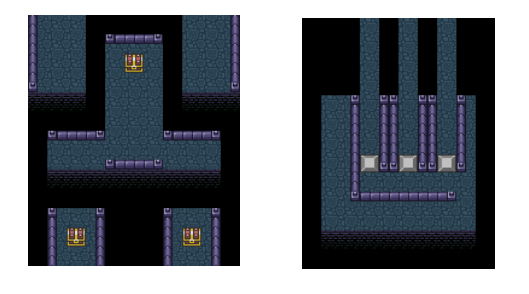
\includegraphics[scale=0.8]{proof1.png}
        \caption{Dispositivos de variável e cláusula, respectivamente}
    \end{figure}
    
    O dispositivo de cláusula é ilustrado também na figura 4. Os três corredores de cima correspondem aos literais que aparecem
    na cláusula. Quando link visita um desses corredores, ele deve empurrar o bloco para frente, o que permite a ele 
    utilizar o gancho em um dos blocos da direita depois, quando estiver atravessando o caminho de checagem (figura 5).
    Note que a barreira mais a esquerda do dispositivo de cláusula previne Link de "pular" clausulas não satisfeitas, mesmo
    se ele puder usar o gancho arbitrariamente a longas distâncias.
    
    \begin{figure}[!htb]
        \centering
        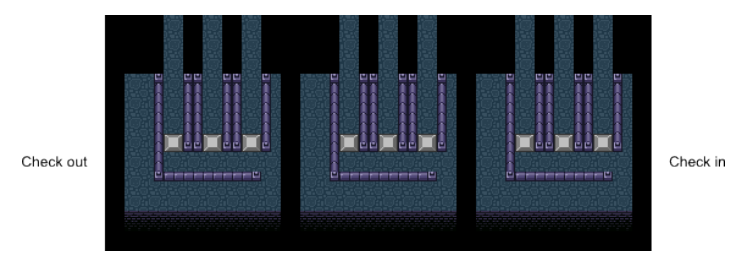
\includegraphics[scale=0.7]{proof2.png}
        \caption{Caminho de checagem}
    \end{figure}
    
    Por fim, o dispositimo de crossover já é nativamente implementado no jogo, como mostra a figura 6.
    
    \begin{figure}[!htb]
         \centering
         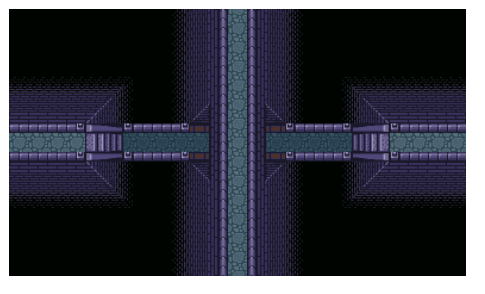
\includegraphics[scale=0.7]{proof3.png}
         \caption{Dispositivo de Crossover}
    \end{figure}
    
\end{proof}

\subsection{NP}

\newtheorem*{theorem2}{Teorema 2}

\begin{theorem2}
    Decidir quando uma posição final é alcançável a partir de uma dada posição
    inicial em uma versão generalizada de The Legend Of Zelda: A Link to the Past é NP.
\end{theorem2}

\begin{proof}
    Para concluir a prova da NP-Completude de Zelda, basta provarmos que finalizar o jogo é um problema NP.
    Se mostrarmos um caminho que é sempre possível,
    então há um algoritmo de solução de localização de caminho com um tempo de execução que é
    no máximo polinomial no tamanho da entrada, ou seja,
    podemos mostrar por certificados que o problema é verificável em tempo polinomial, o que por definição o torna um problema NP.
    
    Então, suponde que existe tal solução, vamos considerar qualquer caminho que Link pode fazer no mapa.
    Uma vez que só é possível abrir os baús que contém itens únicos do jogo uma vez, e que se matarmos
    todos os inimigos pelo menos uma vez teremos matado todos os inimigos que soltam itens especiais e também o chefe final do jogo, podemos dizer que
    o caminho que passa por cada um dos baús atualmente alcançáveis, e elimina cada um dos inimigos alcançáveis
    uma vez (lembrando que todos os inimigos podem ser derrotados desde o primeiro momento do jogo), então
    existe uma solução polinomial ao tamanho da entrada.
    
    Tal demonstração é similar as feitas por \cite{gabrielsen2012video} para outros jogos da Nintendo
    (Super Mario Bros., Donkey Kong Country e Metroid).

\end{proof}    

